% ----------------------------------------------------------------------
% ----------------------------------------------------------------------

\documentclass[
    aps, 
    twocolumn, 
    secnumarabic, 
    balancelastpage, 
    amsmath, 
    amssymb, 
    nofootinbib, 
    floatfix
]{revtex4-2}

% ----------------------------------------------------------------------

\usepackage{graphicx}      
\usepackage{lgrind}        
\usepackage{xcolor}            
\usepackage{epsf}       
\usepackage{bm}          
\usepackage{asymptote}     
\usepackage{thumbpdf}
\usepackage[colorlinks=true]{hyperref} 
\usepackage{physics}
\usepackage{enumerate}
\usepackage{enumitem}
\usepackage{caption}
\usepackage{subcaption}

% ----------------------------------------------------------------------

\begin{document}
\title{Estimating the Mean Lifetime of a Muon}
\author{Perrin W. Davidson}
\email{pwd@uchicago.edu}
%\homepage{https://perrinwdavidson.github.io/perrin/}
\date{\today}
\affiliation{UChicago Department of Physics}

% ----------------------------------------------------------------------

\begin{abstract}

By observing the time between the arrival of short-lived muons and their subseqeuent decay into electrons, we determine the mean lifetime of muons by fitting the time distribution using the Levenberg-Marquardt algorithm implementation of generalized non-linear least squares. We find the scaled mean muon lifetime to be $\tau = 2.21 \pm 0.04 \times$ $\mu$s, which is in agreement with previously published literature value of $2.20$ $\mu$s, within uncertainty. We correspondingly determine the Fermi coupling constant to be $\text{G}_F/(\hbar c)^3 = (1.16 \pm 0.01) \times 10^{-5}$ GeV$^{-2}$. We find that our value for the Fermi coupling constant also agrees with previously published literature value of $1.16 \times 10^{-5}$ GeV$^{-2}$.   

\end{abstract}

% ----------------------------------------------------------------------

\maketitle

% ----------------------------------------------------------------------
% ----------------------------------
\section{Introduction}
\label{sec:intro}

Muons ($\mu^-$) and antimuons ($\mu^+$) are unstable lepton particles with charges $^-e$ and and $^+e$, respectively. Both particles are produced from the interactions between high energy cosmic particles (high-energy photons) and atmospheric particle nuclei in the upper atmosphere, between 10 to 20 km above sea level \cite{manual2021}. Muons decay into electrons, nutrinos, and antinutrinos while antimuons decay into positrons, nutrinos, and antinutrinos. These particles therefore decay following:
\begin{equation}
	\mu^\pm \rightarrow e^\pm + \nu + \bar{\nu},
	\label{eq:muonDecay}
\end{equation}
where $e^\pm$ is an electron or positron (antielectron), $\nu$ is a nutrino, and $\bar{\nu}$ is an antinutrino. \par

The interactions between air nuclei and cosmic particles create showers of muons, antimuons, gamma rays, and other charged particles, where the production of muons and antimuons are to nearly the same number. For an incident rate $R_0$ of (anti)muons showering earth, we can break down this as a sum of both charged particle follwing:
\begin{equation}
	R_0 = R_0^+ + R_0^-,
	\label{eq:coeffs}
\end{equation}
for $R_0^+$ the incident rate of antimuons and $R_0^-$ is the incident rate of muons. Therefore, we can prescribe a percentage of $R_0$ attributed to both the muon and antimuon such that $R_0^+ = 0.56R_0$ and $R_0^- = 0.44R_0$ \cite{galbiati2005}. \par 

Given the similarity of the production of muons and antimuons, the detection of either charged particle will lead to an execptable estimate on the muon mean lifetime. The lifetime of a muon is $2.196981 \pm 0.000002 \times 10^{-6}$ seconds. The mass of a muon is over 200 times that over an electron ($m_e = 0.511$ MeV c$^{-2}$) and given as $m_\mu = 105.7$ MeV c$^{-2}$ \cite{olive2014, manual2021}. It is important to note that given this short mean lifetime, a muon produced in the upper atmosphere traveling at almost the speed of light would not reach the earth's surface. It is only after considering the relativistic time dilation that muons are able to reach the earth's surface \cite{manual2021}. \par  

As muons and electrons are charged particles, we know that any interactin they will have with matter will involve a deposition of energy into that matter via the Coulomb interaction. A fraction of this deposited energy will be in the form an initial pulse of light. If we consider this matter to be a scintillator of the form that is used in our experiment, then we have a method by which to observe the impact of the muon with the scintillator. Additionally, the decay of the muon into the electron will generate a second pulse of light. This is an idealized case, and for any muon traveling within the scintillator, the pulse of lightwill be percieved by instrumentation as a single flash. Despite this, the distribution of the delay between the discrete first and second pulses of light for a large ensemble of muon particles allows us to determine the mean lifetime of a muon and forms the basis of our experimental design.

By utilizing this knowledge of the muon decay processes and interaction with media, we can estimate the mean lifetime of a muon from the its observed decay time into electrons, following Eq. \eqref{eq:muonDecay}. We then use this mean lifetime to calculate the Fermi coupling constant. 

% ----------------------------------
% Experimental Setup
% ----------------------------------
\begin{figure*}[t]
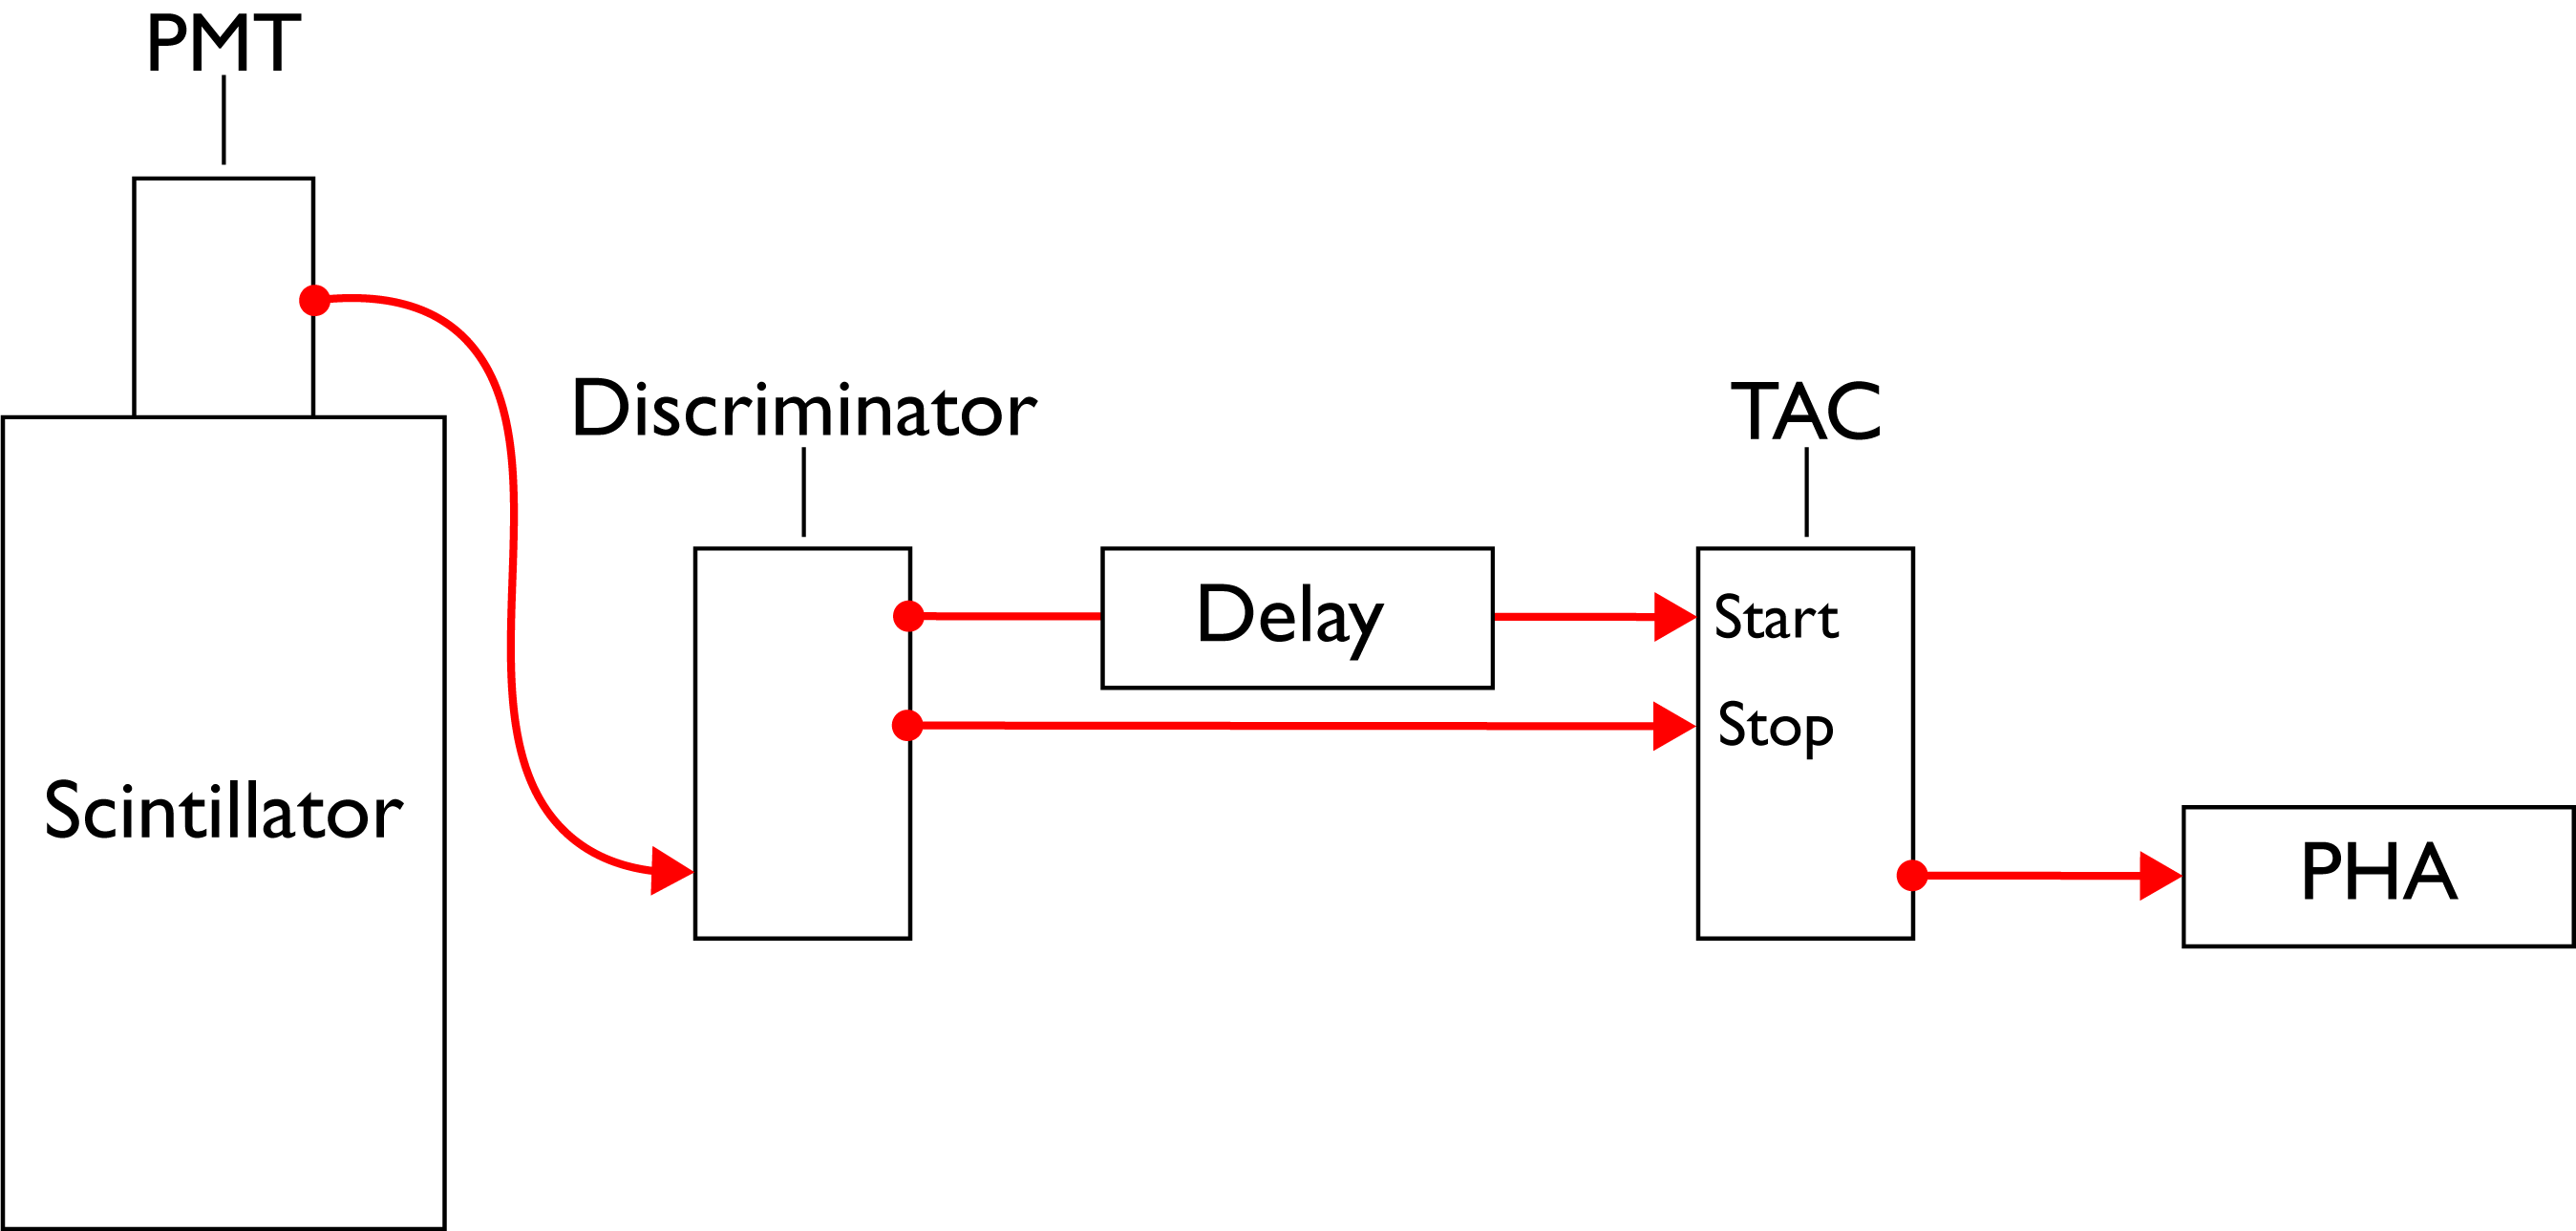
\includegraphics[width=12cm]{figures/expSetup.png}
\caption{Experimental setup employed to detect muon decays in an organic scintillator. The decay of muons into electrons within the organic scintillator follow the red arrows.}
\label{fig:exp_setup}
\end{figure*}
% ----------------------------------

% ----------------------------------
\section{Theory}

% ----------------
\subsection{Modeling Muon Decay}
\label{sec:timeModel}

Let us consider an ensemble of muon particles where the initial size $N_0$ is large. Then, assuming that count rates $R$ are proportional to the remaining number of particles in our ensemble $N$, we can describe the decay of this large of muon ensemble into electrons and (anti)nutrinos following the exponential: 
\begin{equation}
	R(t) = R(t = 0) e^{-t/\tau},
	\label{eq:expDecay}
\end{equation}
where $\tau$ is known as the ``e-folding'' time scale as it is the time that it takes for our ensenble to fall to $1/e$ of it's initial size $N_0$. Therefore, we can view Eq. \eqref{eq:expDecay} as modeling the expected rate of muons at sea level. \par 

Now, from our discussion of exponential decay of uons and Eq. \eqref{eq:expDecay}, we can see that the muon decay process can be modeled by the exponential distribution. Making the assumption that the exponential decrease in muon flux is due to muon decay, we can then model the muon decay with the probability distribution: 
\begin{equation}
	P(t) = P(t = 0)e^{-t/\tau},
\end{equation}
which allows us to view $\tau$ as the mean lifetime of a muon, given that it is the expectation of the exponential distribution. \par

In order to obtain $\tau$, the mean lifetime, we want to fit an observed spectrum of muon decay times and extract the fitted expectation of the exponential function. To do this, we will use the objective function:
\begin{equation}
	N(x) = N_0 e^{-x/\tau} + B
	\label{eq:specFit}
\end{equation}
where $x$ is the channel number and $B$ is the background, assumed constant. This is the fundamental equation that allows us to estimate the mean lifetime of a muon.

It is important to note that we need a background term  because we are dealing with the convolution of two exponentials, where the background is one of the exponentials. Therefore, the background is not truly a constant. However, we can assume that it is a constant because by visual inspection of the decay distribution, the e-folding length for the background exponential is large and the amplitude small relative to that of the actual spectrum. Thus, by magnitude comparison, the backgorund term is essentially linear. Additionally, when we consider the distribution of muon decay times in a log scale, which means that we are dealing with a spectrum that appears linear, the difference in linear slope between the background and the distribution of muon decay times is large upon visual inspection, supporting our assumption that we can basically consider the background constant.

% ------------------
\subsection{Weak Interactions}
\label{sec:fermiConstant}

Muon decay only invovles the weak interaction, one of the four fundamental forces along with electromagnetic, strong, and gravitational forces. It is one of the only such processes that exist in nature where only the weak interaction is invovled. Therefore, we can view muon decay and the mean lifetime as a measurement of the magnitude of the weak interaction. In the context of our experiment, we will use our measured mean lifetime with the Fermi coipling constant, $G_F$, to quantify the magnitude of the weak interaction. Specifically, the Fermi coupling constant is given as: 
\begin{equation}
	\dfrac{G_F}{\left(\hbar c\right)^3} = \sqrt{\dfrac{192\pi^3\hbar}{\left(m_\mu c^2\right)^5\tau}}.
	\label{eq:fermi}
\end{equation}

The literature value of the Fermi coupling constant is given as $G_F/(\hbar c)^{3} =  1.1663787 \pm 0.000 0006 \times 10^{-5}$ GeV$^{-2}$ \cite{nistFermi}.  

% ----------------------------------
\section{Methods and Materials}

% ---------------
\subsection{Experimental Setup}
\label{sec:expSetup}

Our experimental setup is presented in Fig. \ref{fig:exp_setup}. As discussed in Section \ref{sec:intro}, our experimental procedure measures the time distribution of the delay between two light pulses emitted from muons impacting our scintillator and decaying into electrons. As shown in Fig. \ref{fig:exp_setup}, the scintillator is where our procedure begins. Specifically, we use a metal oil drum filled with mineral oil as a liquid organic scintillator to detect muon decay. This scintillator is similar to NaI crystal-type detectors in that it is the light pulse given off by the high energy particle collision with the matter of the scintillator -- whether that be solid NaI crystal or liquid mineral oil -- which is measured in the experiment. We use a 41 cm diameter by 61 cm high cylindrical metal drum as our scintillator, painted white on the interior. The matter within the drum is an organic chemical dissolved in oil.  

These light pulses emiited from the ionizing radiation of the muon impacting the mineral oil of the scintillator and subsequent decay into electronsd are measured by a photomultiplier tube (PMT). This 13 cm diameter instrument is mounted on top of the scintillator and emits a charge pulse when it sees a light pulse in the scintillator. The high voltage setting for the PMT was set to -1800 V. This value was chosen to best amiply the desired muon and electron pulses above the threshold while keeping the noise pulses below the threshold. This choice represents the best trade off between a higher count rate and more noise. It is important to note the sources of pulses that the PMT will measure. One source is the scintillation light from muons moving through the scintillator. Along with the scintillation light from decay electrons, these represent the sources we aim to measure. A third source is that of other particles moving through the scintillator but not decaying, and a final source is that of noise pulses, which originate from within the PMT when electrons are ejected from the PMT photo-cathode. 

These charge pulses are sent to the discriminator which performs two functions. First, the discriminator only accepts PMT charge pulses that are greater than a constant threshold. The aim of this function is to minize the number of noise pulses that we detect, as described above in the sources of scintillation light detected by the PMT. When a PMT charge pulse is greater than this threshold, the disciminator produces a uniform output pulse of -0.7 V with a width of 10 ns, chosen to be optimal for the subsequent instruments. For our experiment, this threshold was set -30.2 mV. Visual inspection through an oscilloscope showed that this threshold was sufficient in minimizing the number of noise pulses detected ($>-10$mV), leaving only the larger, less frequent pulses being detected. The disciminator has two ouput channels. One of these is delayed via a delay box, which delays the uniform pulse from the disciminator for a set time length. Our delay was set to $50 \pm 0.1$ ns. The delay box is crucial to our experimental setup, and our configuration of delayed input as the start and non-delayed discriminator pulse as the stop is the only correct implementation, as otherwise we would only measure the delay from the delay box. Additionally, this delay will only affect the exponential distribution discussed in Section \ref{sec:timeModel} by multiplying a constant proportional to $\exp[50\text{ns}]$ to the initial rate $R_0$, which we can deal with appropriately through proper fitting of the exponential distribution.

Following Fig. \ref{fig:exp_setup}, there are two inputs into the next instrument: the TAC. This instrument measures the time between the start and stop pulses from the discriminator. The start pulse is the delayed signal from the discriminator. The stop pulse is the unaffected output channel from the disciminator. The TAC then produces an output pulse which has a height proportiomal to the measured time difference between the start and stop pulses. It is important to note that the TAC has a range of 20 $\mu$s, which means that if a time difference is greater than this setting, the TAC resets without producing an output pulse. This is an instrumentational constrain on our measurement of the muon decay time into electrons. 

The TAC output pulse is then read and binned by the spectrometer pulse height analyzer (PHA). The PHA sends this data to a computer, where the USX program displays a histrogram of counts per channel. Our conversion gain was set to 512. Therefore, there were 512 channels into which the TAC output is binned, with each channel being proportional to time, specifically the decay time of muons into electrons. 

There are four additional instruments that should be discussed. The first two instruments are the scaler and timer, where the scaler is used to count the pulses from the disciminator over a set time duration controlled by the timer. To correlate channels to time, we used a double pulser. This instrument produces pulse pairs that simujlate the PMT pulses from muon-electron pairs. In conjuction with an oscilloscope, we measured the time difference between each pulse pair on an oscilliscope, given us a measurement of time, to which we correlated the corresponding channel output from the PHA/OSX binning.   

This experimental setup was used to detect the decay of muons into electrons in our experiment. It was run for 249174.29 seconds, or approximately 69 hours. During this time, 20880 events were collected. 

% ---------------
\subsection{Time Calibration}
\label{sec:timeCal}

Noting that the independent variable in Eq. \eqref{eq:specFit} is channel number, which is due to our experimental set-up described in Section \ref{sec:expSetup}, we need to calibrate our fitted parameter $\tau$ from units of [CHANNEL] to units of [TIME]. To do this, we will perform a linear fit of channel number to known delay time using:
\begin{equation}
	D(x) = mx + b
	\label{eq:timeCalFit}
\end{equation}
where $x$ is the channel number.

To calculate the final mean lifetime, we evaluate Eq. \eqref{eq:timeCalFit} at $x = \tau(\text{[CHANNEL]})$, neglecting the y-intercept, to get the decay time, $D = \tau([\text{TIME}])$, in units of time. Explicitly, this is given by:
\begin{equation}
	\tau = D(\tau(\text{CHANNEL}))\big\lvert_{b=0}.
	\label{eq:timeConvert}
\end{equation}
It is important to note that we ran this conversion before and after the 69 hour collection period. To best represent any change in calibration over this time, both sets of calibration data were fit and the average fit value of $m$ was determined as the conversion factor to convert our mean lifetime of a muon from units of channels to units of time. The average was taken to represent the mean change in conversion over the time of the experiment. 

The error, denoted with a $\delta$, in this calculation is then found using the equation:
\begin{equation}
	\delta \tau = \sqrt{(\delta mx)^2 + (\delta x m)^2},
	\label{eq:timeConvertErr}
\end{equation}
following the generic error propogation formula:
\begin{equation}
	\delta f(x, \cdots, z) = \sqrt{\left(\pdv{f}{x}\delta x\right)^2 + \cdots + \left(\pdv{f}{z}\delta z\right)^2}.
	\label{eq:errorProp}
\end{equation}

Explicitly, the average was taken, for subscripts 1 and 2 denoting Days 1 and 2, respectively:
\begin{equation}
	m = \dfrac{m_1 + m_2}{2},
	\label{eq:timeConvertCalc}
\end{equation}
where the corresponding error is given as:
\begin{equation}
	\delta m = \sqrt{\left(\dfrac{\delta m_1}{2} \right)^2 + \left(\dfrac{\delta m_2}{2} \right)^2}.
	\label{eq:timeConvertCalcErr}
\end{equation}
Here we used Eq. \eqref{eq:errorProp}. 

% -------------------
\subsection{Accidental Count Rate}
\label{sec:accidentRate}

There is some probability that two uncorrelated pulses occure within the PHA range window $T$ and serve as the start and stop pulses within this window, despite the average time betwen pulses being larger than this window. We can model this probability by a Poisson distribution:
\begin{equation}
	P(t)\text{d}t = Re^{-RT}\text{d}t, 
\end{equation}
where $R$ is the overale singles rate of muons. Therefore, we can find the total expected accidenta rate of starting and stoping with uncorrelated muons with the PHA range to be:
\begin{align}
	R_{acc} &= R\displaystyle\int_{0}^{T} P(t) dt \\ 
		&= R \displaystyle\int_{0}^{T} Re^{-Rt}dt \\ 
		&= R\left(1-e^{-RT}\right).
\end{align}
Then, we approximate this accidental rate for $e^{x} \approx 1 + x + \cdots$ in the limit of $T \ll 1/R$, giving:
\begin{equation}
	R_{acc}\approx R^2T.
	\label{eq:raccExp}
\end{equation}
The error for this calculation is then:
\begin{equation}
	\delta R_{acc} = \sqrt{\left(2RT\delta R \right)^2 + \left(R^2\delta T\right)^2},
	\label{eq:raccExpErr}
\end{equation}
following Eq. \eqref{eq:errorProp}. 

Now, Eq. \eqref{eq:raccExp} constitutes the expected accidental count rate. To calculate the experimental accidental count rate, we will use the following equation:
\begin{equation}
	R_{acc}^{\**} = \dfrac{B\lvert \bm{y} \rvert}{\Delta t},
	\label{eq:raccAsc}
\end{equation}
where $B$ is the background fit parameter in Eq. \eqref{eq:specFit} representing the number of background counts present in each of the channels, $\bm{y}$ is the array of all channels in the histogram of muon decay times and $\lvert \cdot \rvert$ is the number of data points (cardinality) in this vector, and $\Delta t = 249174.29 \pm 1$ seconds is the total runtime of our experiment. The error associate then with this calculation is, following Eq. \eqref{eq:errorProp}:
\begin{equation}
	\delta R_{acc}^{\**} = \sqrt{\left(\dfrac{\lvert\bm{y}\rvert}{\Delta t} \delta B\right)^2 + \left(\dfrac{B}{\Delta t} \delta\lvert\bm{y}\rvert\right)^2 + \left(\dfrac{B\lvert\bm{y}\rvert}{(\Delta t)^2} \delta\Delta t\right)^2}.
	\label{eq:raccAscErr}
\end{equation}

% -----------------
\subsection{Muon Environment Correction}
\label{sec:muonCorrect}

Given the discussion in Section \ref{sec:intro}, we know that there are multiple decay paths for muons. For the positive muons, there is only one path, namely the decay into electrons. However, for the negative muons, in addition to decaying into electrons, these particles can also mimic an electron and be captured by an atom of the scintillator. This then may interact to convert a proton into a neutron of this atom, giving
\begin{equation}
	\mu^-+p\rightarrow n+\nu.
\end{equation}
We can model this by calculating an absorption time constant, which we will call $\tau_{abs}$. Then, the decay constant that we will estimate from our muon decay histogram is a composite of these two processes: 
\begin{equation}
	\dfrac{1}{\tau_{meas} }= \dfrac{1}{\tau} + \dfrac{1}{\tau_{abs}}.
\end{equation}
This means that in the context of our experiment, where $\tau_{abs}$ is much larger than $\tau$, the measured time constant, $\tau_{meas}$, is $4\%$ lower than the the free muon lifetime. Therefore, we must multiply our fitted parameter by a constant, $\alpha = 1.04$ in order to account for this and estimate an accurate mean lifetime. This gives us the equation to determine our final, scaled mean lifetime of a muon as:
\begin{equation}
	\tau = \alpha\tau_{meas}.
	\label{eq:tauCorrect}
\end{equation}
The error for this calculation is then:
\begin{equation}
	\delta \tau = \alpha \delta \tau_{meas}.
	\label{eq:tauCorrectError}
\end{equation}

% ----------------------------------
% Observed Spectrum
% ----------------------------------
\begin{figure*}[t]
	\centering
     	\begin{subfigure}[t]{12cm}
         	\centering
		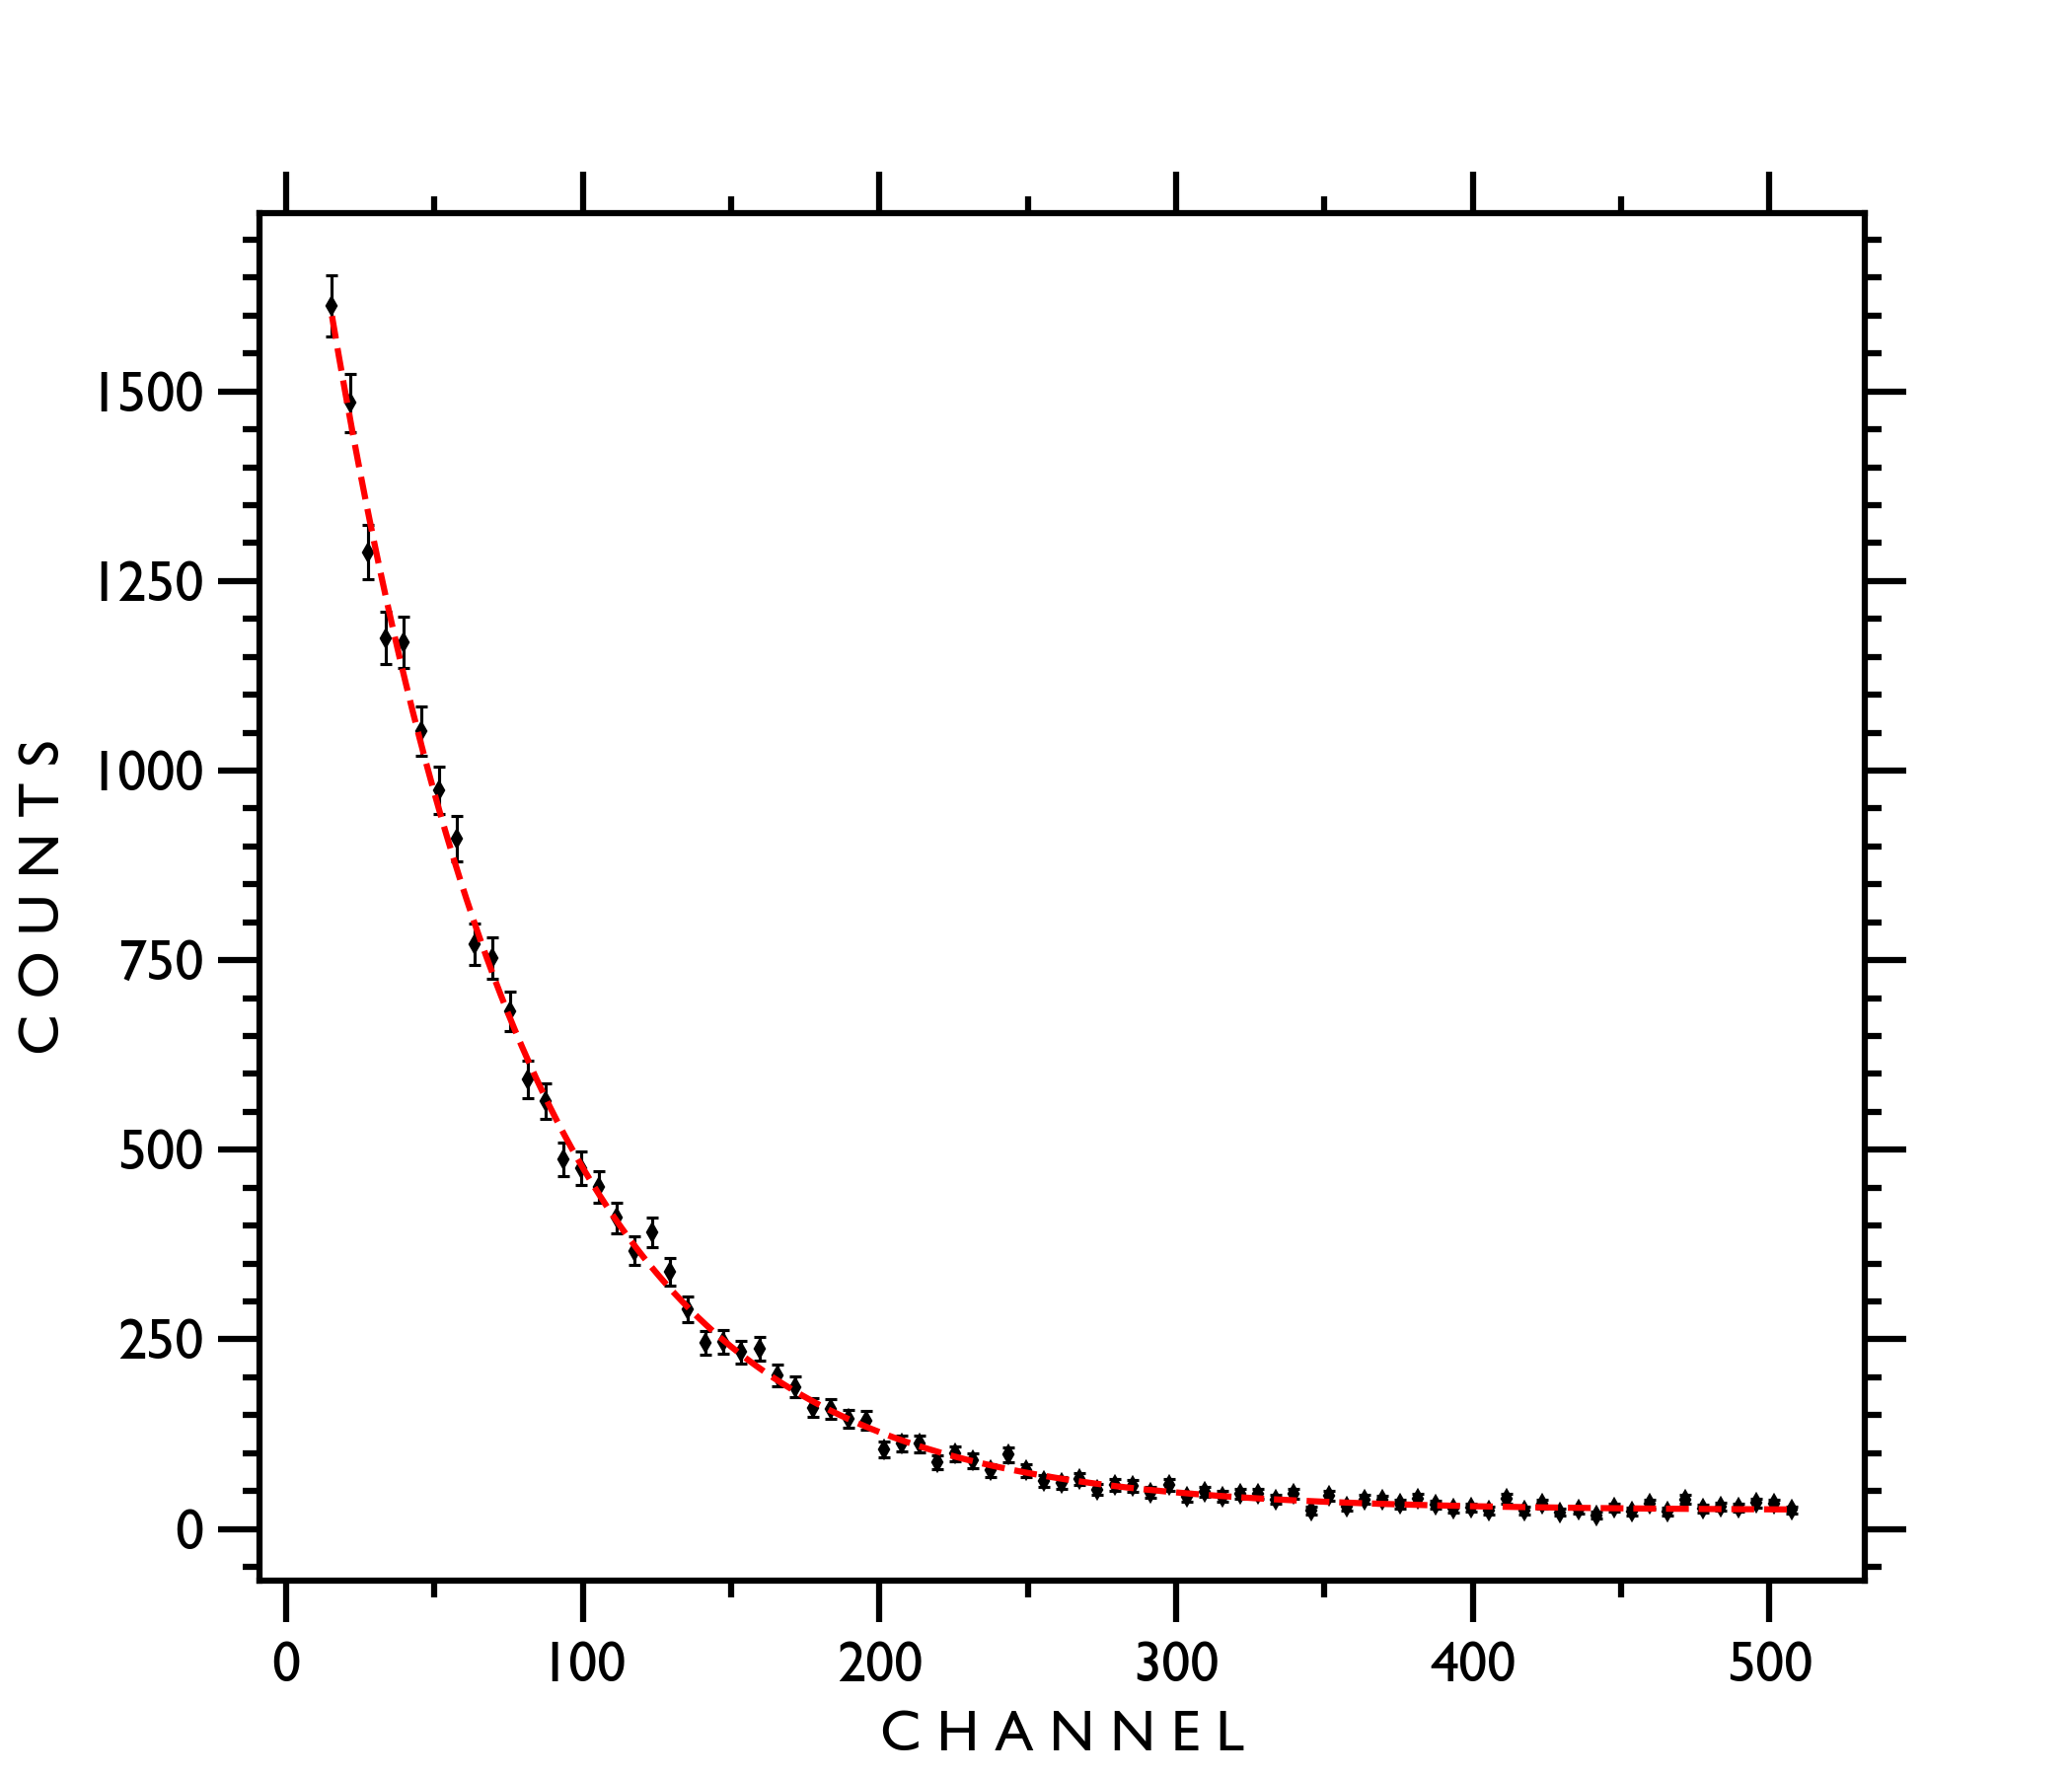
\includegraphics[width=12cm]{figures/muon_spectrum.png}
	\end{subfigure}
	\\
	\bigskip
	\begin{subfigure}[t]{12cm}
         	\centering
		\begin{tabular}{c|c}
            	\textbf{Fit Parameter} & \textbf{Value} \\
            	\hline
            	$N_0$ (counts) & $1.98 \times 10^{3} \pm 26$ \\ 
            	$\tau$ (channel) & $67.7 \pm 0.7$  \\
	    	$B$ (counts) & $24.6 \pm 1.0$  \\
		\end{tabular}
     	\end{subfigure}
     	\\
     	\bigskip
     	\begin{subfigure}[t]{12cm}
         	\centering
		\begin{tabular}{c|c}
            	\textbf{GoF Parameter} & \textbf{Value} \\
            	\hline
            	$\chi^2$ & $83.5$ \\ 
            	$N_\nu$ & $80.0$  \\
	    	$\chi^2_\nu$ & $1.04$ \\
		\end{tabular}
     	\end{subfigure}
     	\bigskip
	\caption{Observed spectrum and corresponding exponential fit of muon decay times collected over a 69 hour period. The black diamonds are the observed muon decay times through the experimental setup described in Section \ref{sec:expSetup} with associated error bars in black. The dashed red line is the exponential function fit described in Eq. \eqref{eq:specFit} through the Levenburg-Marquadt algorithm implementation of non-linear least squares described in Section \ref{sec:fitting}. The upper table presents the fit parameters for those parameters in Eq. \eqref{eq:specFit}. The lower table presents the goodness of fit (GoF) parameters for the fit.}
	\label{fig:muon_spectrum}
\end{figure*}
% ----------------------------------

% ----------------------------------
% Time Calibration
% ----------------------------------
\begin{figure*}[t]
	\centering
     	\begin{subfigure}[t]{12cm}
         	\centering
		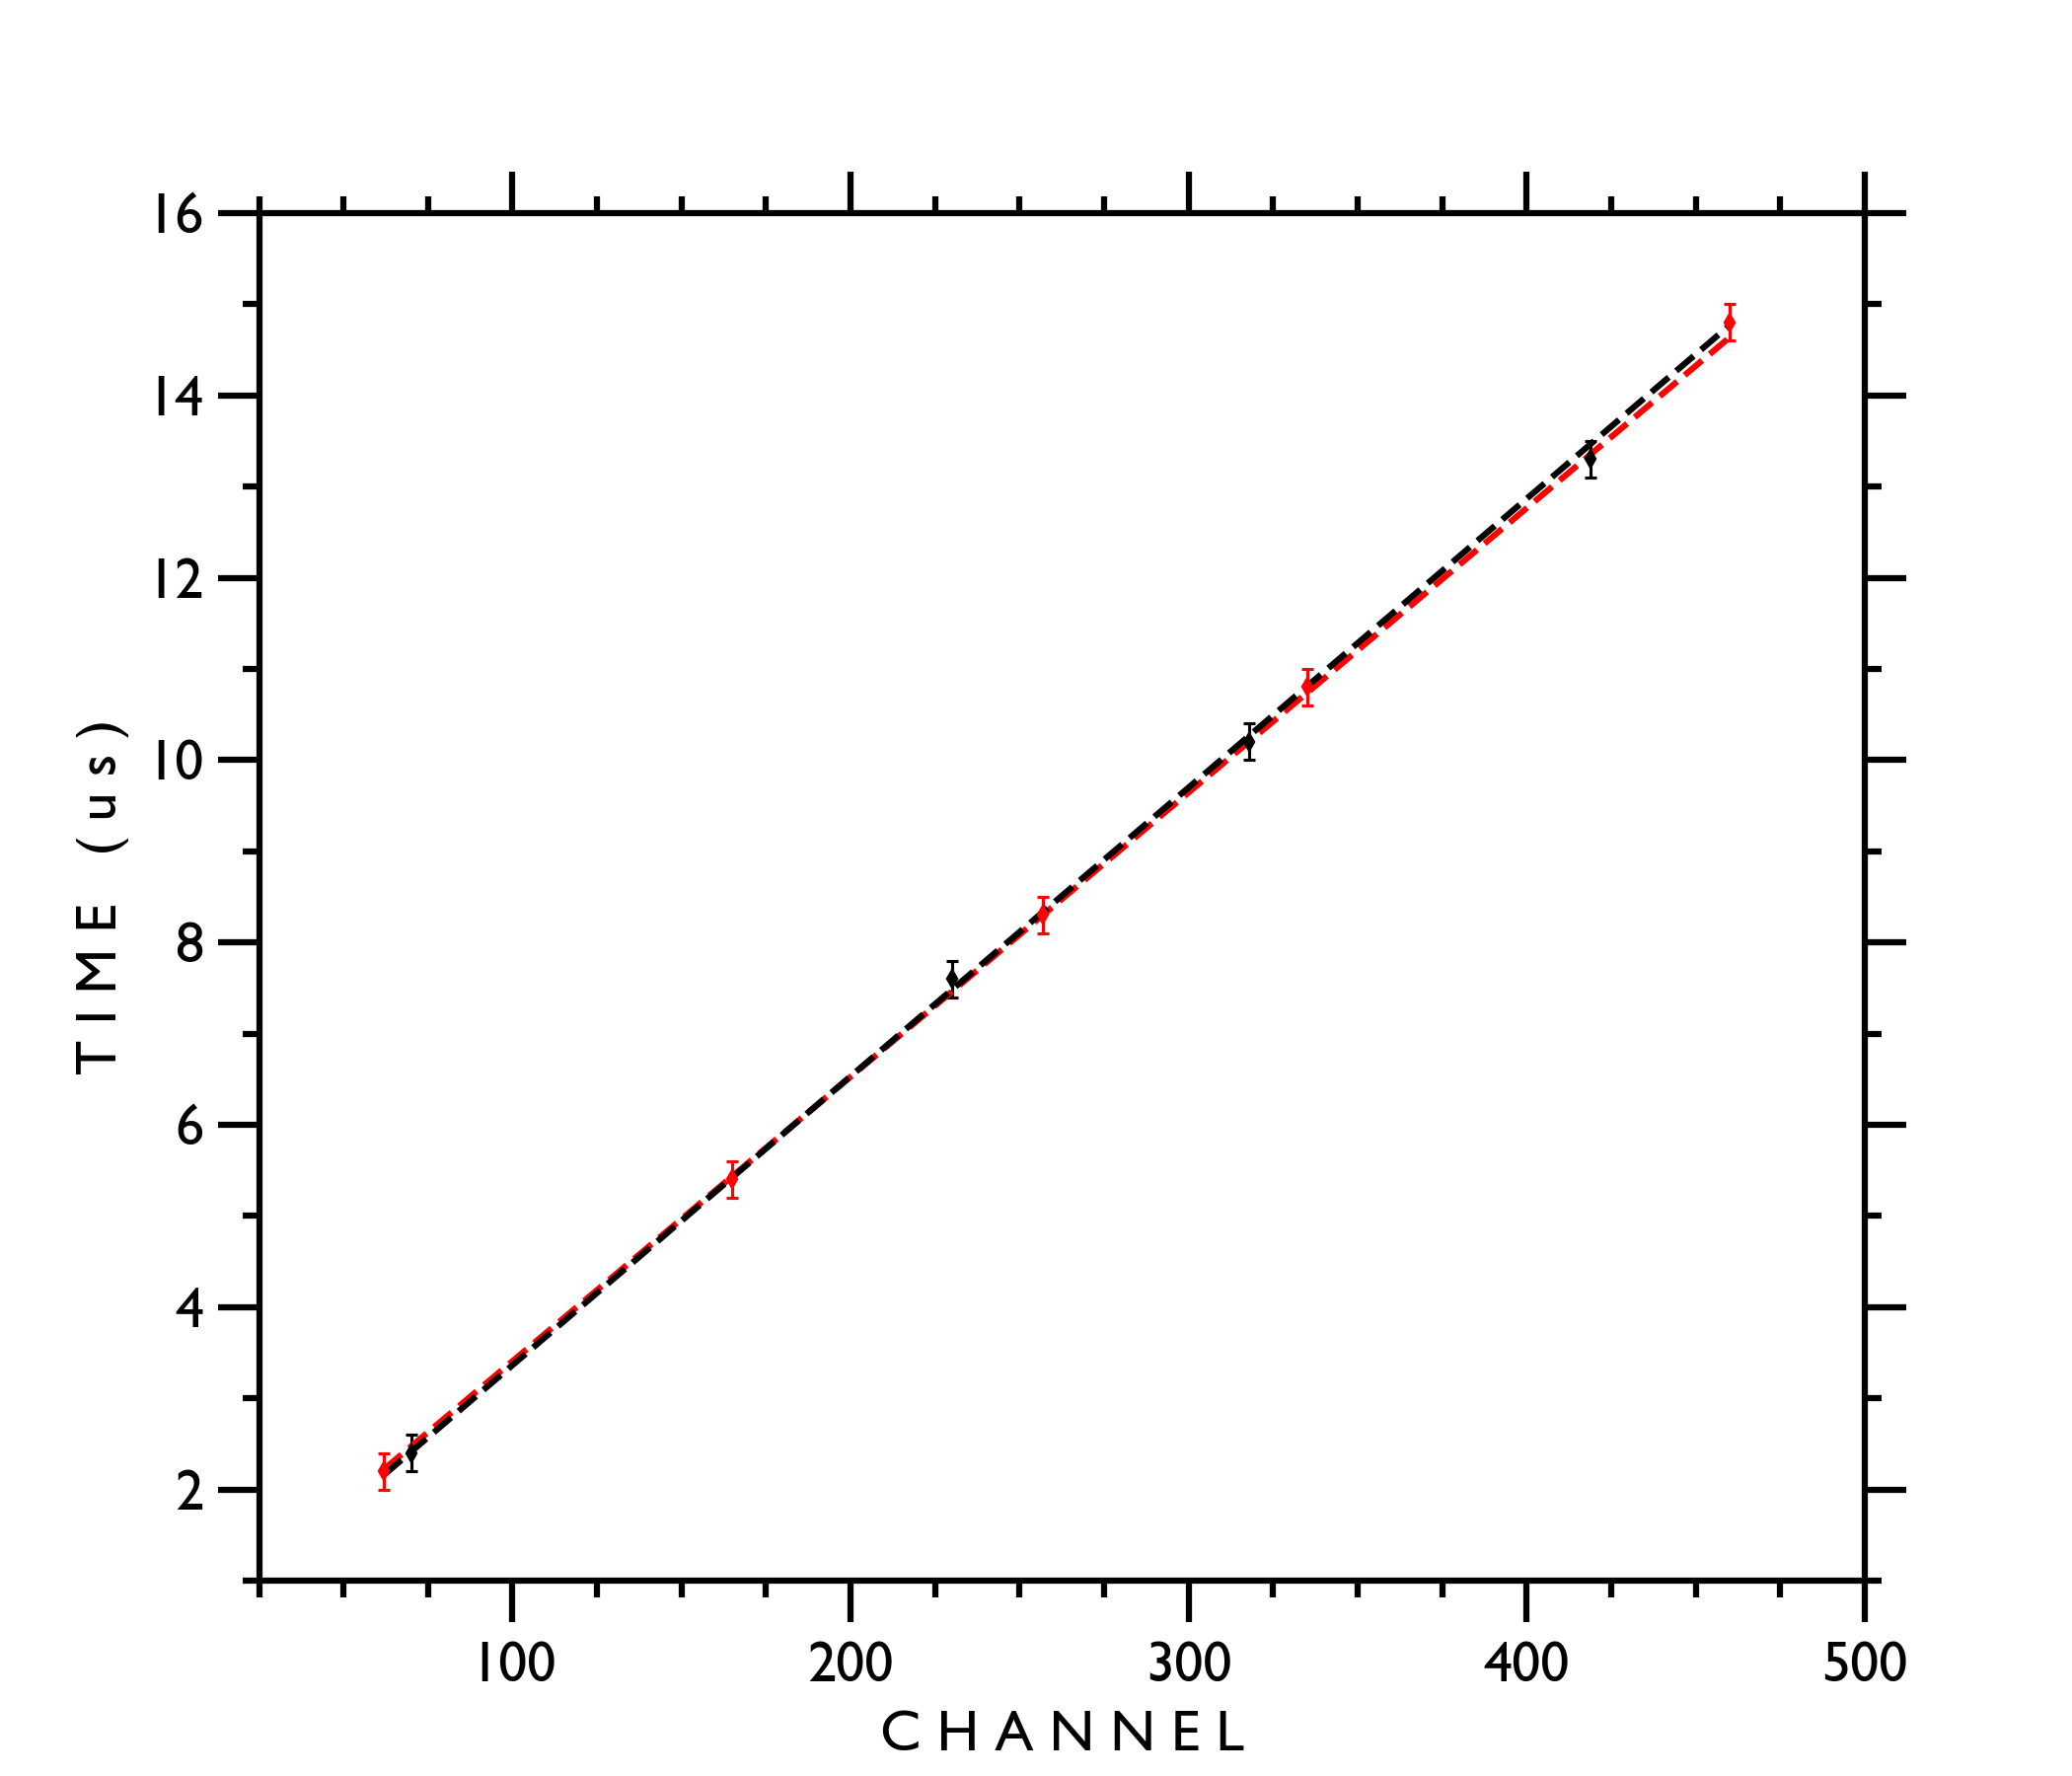
\includegraphics[width=12cm]{figures/time_calibration.png}
	\end{subfigure}
	\\
	\bigskip
	\begin{subfigure}[t]{12cm}
         	\centering
		\begin{tabular}{c|cc}
              		\textbf{Fit Parameter} & \textbf{Day 1} & \textbf{Day 2} \\
            		\hline
	    		$m$ (counts/channel) & $ 0.3119 \pm 0.0008 $ & $0.3168 \pm 0.0007$ \\
	    		$b$ (counts) &  $0.2889 \pm 0.2257$ & $0.1962 \pm 0.1895$ \\
		\end{tabular}
     	\end{subfigure}
     	\\
     	\bigskip
     	\begin{subfigure}[t]{12cm}
         	\centering
		\begin{tabular}{c|cc}
	    		\textbf{GoF Parameter} & \textbf{Day 1} & \textbf{Day 2} \\
            		\hline
	    		$\chi^2$ & $0.69$ & $0.12$ \\ 
	    		$N_\nu$ & $2.0$ & $3.0$ \\
	    		$\chi^2_\nu$ & $0.34$ & $0.04$ \\
		\end{tabular}
     	\end{subfigure}
     	\bigskip
	\caption{PHA channel to delay time calibration taken the first (1) and last (69) hour of muon decay collection. The black diamonds are measured channel to delay times for the first hour, with the corresponding error bars in black. The dashed black line is the linear fit presented in Eq. \eqref{eq:timeCalFit}. The red diamonds are the measured channel to delay times for the last hour (hour 69), with associated errors in red. The dashed red line is the linear fit presented in Eq. \eqref{eq:timeCalFit}. The upper table presents the fit parameters presented in Eq. \eqref{eq:timeCalFit}, with the lower table presenting the goodness of fit parameters for this fit.}
	\label{fig:time_calibration}
\end{figure*}
% ----------------------------------

% -----------------
\subsection{Non-Linear Least Squares Fitting Routine}
\label{sec:fitting}

To estimate the mean lifetime of muons $\tau$ in this experiment, we use a generalized, non-linear least squares method. The function fit to the estimated Poisson Distribution from Sec. \ref{sec:timeModel} is Eq. \eqref{eq:specFit}, as it is a generalized form of the theoretical, power law-derived equations for both regimes. The uncertainties for the least-squares parameters $N_0, \tau$ and $B$ as presented in Eq. \eqref{eq:specFit} were calculated from the Levenberg-Marquadt algorithm implementation of this least squares method. The method works to minimize the squared sum of the fit residuals normalized by the uncertainty, $\epsilon$:
\begin{equation}
    \chi^2 = \sum_{i=1}^{N-1} \left(\frac{\widehat{y}_i - y_i}{\epsilon_i}\right)^2,
    \label{eq:chiSquared}
\end{equation}
where $\widehat{y}_i$ is the fit value and $y_i$ the measured value. The uncertainty in each estimated parameter is determined by the variance in the parameter estimate, given generically for a parameter function $\Theta(\bm{x})$ by \cite{manual2021_lsm}:
\begin{equation}
    \sigma^2_\Theta = \sum_{t=0}^{N-1} \sigma^2_i\left(\dfrac{\partial \Theta}{\partial x_i}\right)^2
\end{equation}
where $x_i \in \bm{x}$ are the parameters being fit and $\sigma^2_i$ the variance in each parameter fit.
The $\chi^2$ goodness of fit statistic was calculated following :
\begin{equation}
    \chi^2 = \sum_{i=1}^N \left(\frac{\widehat{y}_i - y_i}{\epsilon_i}\right)^2,
\end{equation}
similar in construction to Eq. \eqref{eq:chiSquared}.
The Degrees of Freedom were calculated following:
\begin{equation}
    N_\nu = \lvert \bm{y} \rvert - \lvert \bm{x} \rvert,
\end{equation}
where $\lvert \bm{y} \rvert$ are the data points (response variable) vector being fitted and $\lvert \bm{x} \rvert$ are the numer of parameters being fitted.

% ----------------------------------
% Mean Lifetime and Accident Rate
% ----------------------------------
\begin{figure*}[t]
	\centering
	\begin{subfigure}[t]{4cm}
         	\centering
		\begin{tabular}{c|c}
	    		 & $\bm{\tau}$ ($10^{-6}$s) \\
            		\hline
			Unscaled & $2.13 \pm 0.04$ \\ 
			Scaled & $2.21 \pm 0.04$ \\
		\end{tabular}
     	\end{subfigure}
	\hspace{1mm}
     	\begin{subfigure}[t]{4cm}
         	\centering
		\begin{tabular}{c|c}
			 & $R_{acc}$ (muon min$^{-1}$) \\
            		\hline
			$R_{acc}$ & $0.4944282\pm 0.0000003$ \\ 
			$R_{acc}^{\**}$ & $0.4915668 \pm 0.0217877$ \\
		\end{tabular}
     	\end{subfigure}
	\hspace{1mm}
     	\bigskip
	\caption{The left table presents calculated mean lifetime of a muon, $\tau$. Both values were calculated from a non-linear least squares method. The scaled value takes into considertion the multiple decay paths of the negatively charged muon. The right table presents the calculated experimental, $R_{acc}^{\**}$, and expected, $R_{acc}$, accidental count rates. Values were calculated following the method outlined in Section \ref{sec:accidentRate}.}
	\label{fig:outputs}
\end{figure*}
% ----------------------------------

% ----------------
\subsection{Data Handling}
\label{sec:dataHand}

After visually inspecting our initial data, which included channels 1 to 512 given our gain settings, we only fit Channels 12 to 512. This is because the first few data channels were not within the expected exponential decay of the muon time distribution. We attribute this to random noise binning. 

Additionally, to calculate the errors for the histogram counts of decay times, we assume that the distribution follows a Poisson statistic. Therefore, we calculate the uncertainty in the counts as 
\begin{equation}
	\delta N = \sqrt{N}. 
	\label{eq:nUncert}
\end{equation}
However, this assumption breaks down for $N < 20$. Therefore, we rebin the data, combining 6 consecutive bins and averaging the channel number. In doing this, our minimum bin count number went from 2 counts per bin to 18 counts per bin. Therefore, we increase the bin count number to a count where our statistical assumption does not break down, providing assurance to our assumption. 

% ----------------------------------
\section{Results}

% ----------------
\subsection{Muon Decay Time Distribution}
\label{sec:muonDistResult}

The collected histogram of muon decay times is presented in Fig. \ref{fig:muon_spectrum}. The largest bin count is $1613 \pm 40$ at channel 15.5. The smallest bin count is $18 \pm 4$ at channel 441.5. These uncertainties were calculated using Eq. \eqref{eq:nUncert} and the binning was performed following Section \ref{sec:dataHand}. The binning reduced the number of channels from 498 to 83. Given the uncertinaty calculation, note that the errorbars scale with the number of counts per bin. 

Additionally, the dashed red line in Fig. \ref{fig:muon_spectrum} is the fitted exponential function presented in Eq. \eqref{eq:specFit} using the Levenburg-Marquardt algorithm implementation of the non-linear least squares method presented in Section \ref{sec:fitting}. The parameters of this fit are presented in the upper table of Fig. \ref{fig:muon_spectrum}. From these, we are able to extract the unscaled mean lifetime of a muon as $67.7 \pm 0.07$ (channels). The amplitude is found to be $N_0 = 1.98 \times 10^3 \pm 26$ (counts) and the background is found to be $24.6 \pm 1.0$ (counts). The Goodess of Fit metric $\chi^2$ is calculated as $83.5$. For degrees of freedom taken to be $80.0$, the reduced $\chi^2$ is $1.04$. These values are presented in the lower table of Fig. \ref{fig:muon_spectrum}.   

% ----------------
\subsection{Mean Lifetime Determination}

We followed the procedure presented in Section \ref{sec:timeCal} to calibrate our mean lifetime fitted in units of channels to units of time. Using Eq. \eqref{eq:timeConvert} for the calibration and Eq. \eqref{eq:timeConvertErr} to calculate the error in this calibeation, we get that our unscaled mean lifetime of a muon is $\tau = 2.13 \pm 0.04$ $\mu$s. The goodness of fit metric of $\chi^2$ for the linear fits are $0.69$ and $0.12$ for the first and second day calibration, respectively. Similarly, for degrees of freedom of 2 and 3, the reduced $\chi^2$ for these fits are $\chi^2_\nu = 0.34$ and $0.04$, respectively for the first and second calibration day.

Then, applying the scaling constant and assocaited error calculation presented in Eq. \eqref{eq:tauCorrect} and Eq. \eqref{eq:tauCorrectError}, respectively, we get that the scaled mean lifetime of a muon is $2.21 \pm 0.04$ $\mu$s. These are presented in the left table of Fig. \ref{fig:outputs}.  

% ----------------
\subsection{Accidental Count Rates}

Using the scaler and timer described in Section \ref{sec:expSetup}, we find that the incident rate of muons into the scintillator is $R = 1320 \pm 1$ muon min$^{-1}$. Additionally, we take the error of the PHA window to be $\delta T = 17 \mu$s. Using Eq. \eqref{eq:raccExp} and Eq. \eqref{eq:raccExpErr}, we calculate the expected accidental rate as $R_{acc} = 0.4944282\pm 0.0000003$ (muon min$^{-1}$), respectively. 

We take the error in the channel number to $\delta B = 1$ channel. Then, using Eq. \eqref{eq:raccAsc} and Eq. \eqref{eq:raccAscErr} in addition to the error from the fitted background parameter and the runtime $\Delta t$, we calculate the experimental accidental rate as $R_{acc}^{\**} = 0.4915668 \pm 0.0217877$ (muon min$^{-1}$). The central table of Fig. \ref{fig:outputs} presents these values.

% ---------------
\subsection{Fermi Coupling Constant}

Using Eq. \eqref{eq:fermi} and Eq. \eqref{eq:errorProp}, we can calculate the error of Fermi coupling constant to be generally:
\begin{equation}
	\delta G_f/(\hbar c)^3 = \sqrt{\hbar\dfrac{192\pi^3}{(\mu c^2)^5}} \dfrac{\tau^{-3/2}}{2} \delta\tau.
	\label{eq:gfErr}
\end{equation}
We know that, from Section \ref{sec:intro}, that $\mu c^2 = 105.7$ MeV. We also know that $\hbar = 6.582119569 \times 10^{-16}$ eV s. Then, employing Eq. \eqref{eq:fermi} along with Eq. \eqref{eq:gfErr}, we get that the Fermi coupling consant is $\text{G}_F/(\hbar c)^3 = (1.16 \pm 0.01) \times 10^{-5}$ GeV$^{-2}$. The right table of Fig. \ref{fig:outputs} presents this value.

% ----------------------------------
\section{Discussion}

% -----------------
\subsection{Literature Comparison}

The literature values and the values obtained from our experiment are presented in Table \ref{tbl:lit}. The literature values for the lifetime of a muon is $2.196981 \pm 0.000002 \times 10^{-6}$ seconds \cite{olive2014}. Therefore, as our estimated mean lifetime of a muon is $2.21 \pm 0.04$, our value falls within the literature value within uncertianty.

The literature value of the Fermi coupling constant is $G_F/(\hbar c)^{3} =  1.1663787 \pm 0.000 0006 \times 10^{-5}$ GeV$^{-2}$ \cite{nistFermi}. Therefore, as our estimated Fermi coupling constant is $1.16 \pm 0.01$, our value falls within the literature value within uncertianty.

% -----------------
% Literature Values
% -----------------
\begin{table}[t]
	\begin{tabular}{c|cc}
		\textbf{Parameter} & \textbf{Experiment} & \textbf{Literature} \\
      		\hline
		$\tau$ ($10^{-6}$ s)          & $2.21 \pm 0.04$ & $2.196981 \pm 0.000002$\\
		$G_F/(\hbar c)^3$ ($10^{-5}$ GeV$^{-2}$) & $1.16 \pm 0.01$ & $1.1663787 \pm 0.000 0006$ \\
	\end{tabular}
	\caption{\label{tbl:lit} The literature values of the mean lifetime of a muon and the Fermi coupling constant presented with the values of the mean lifetime of a muon and the Fermi coupling constant obtained from our experiment.}
\end{table}
% -----------------

% -----------------
\subsection{Uncertainties}

It is important to evaluate our use of a single exponential with a constant background term. After measuring with the scaler and timer an incident rate of muons of $R = 1320$ per minute, or 22 muons per second, we can model their arrival by a Poisson distribution of the form seen in Section \ref{sec:accidentRate}:
\begin{equation}
	P(t) = Re^{-RT}.
\end{equation}
Therefore, we can determine the power of the exponent to be on the order of $R = 2.2 \times 10^{-5} (\mu$s$^{-1}$). Given that this equates to an e-folding time scale that is orders of magnitude greater than the incident rate, the order of the difference between teh counts expected between the lowest and highest bins on our historgram are on the order of 200 parts per million. This then means that we can assume that the baseline accidents are constant, as we have in our objective function, Eq. \eqref{eq:specFit}. We find this parameterized background to be $B = 24.6 \pm 1.0$ counts. 

This assumption is further corroborated by our accidental rate calculated as less than 1 accident muon per minute. Additionally, our expected and experimental accidental rates agree within uncertainty, with $R_{acc} = 0.4944282\pm 0.0000003$ (muon min$^{-1}$) and $R_{acc}^{\**} = 0.4915668 \pm 0.0217877$ (muon min$^{-1}$). Given that we are not able to, within uncertainty, say that one muon will accidently fall within our PHA time window, this provides assurance to our experimental method due to the low probability as modeled by the Poisson distribution.  

Our assumption of a single exponential was also checked, by assuming a double exponential of the form: 
\begin{equation}
	N = N_0(0.56e^{x/\tau} + 0.44e^{x/2.043}) + B,
\end{equation}
with the coefficients taken from the discussion of Eq. \eqref{eq:coeffs} and the mean lifetime of the negative muon $\tau = 2.043 \pm 0.04$ $\mu$s taken from \cite{reiter1960}.\footnote{This coefficient was for carbon matter. As our organic liquid scintillator is primarily mineral oil, which is composed of hydrocarbons, this coefficient is adequate given our experiment setup.} The result from this fit was a scaled mean lifetime of $\tau = 2.21 \pm 0.04$ using the same fitting procedure as described previously. This further supports our use of the objective fitting function defined in Eq. \eqref{eq:specFit}. 

% ----------------------------------
\section{Conclusion}

Our experiment falls within the expected literature values for the mean lifetime of a muon and the Fermi coupling constant.  We find the scaled mean muon lifetime to be $\tau = (2.21 \pm 0.04) \times 10^{-6}$ s. We correspondingly determine the Fermi coupling constant to be $\text{G}_F/(\hbar c)^3 = (1.16 \pm 0.01) \times 10^{-5}$ GeV$^{-2}$. This shows that the use of an organic liquid scintillator is a suitable instrument for collecting incident muons. Our experiment also adds to the previous literature by confirming the previous literature values for the mean lifetime of a muon and the Fermi coupling constant. 

Next steps include testing out different scintillator types, sizes, and locations. Determining the environmental affect of the scintillator on this experiment is of primary concern to accurate data collection as we use muons from atmospheric sources.

% ----------------------------------------------------------------------

\begin{acknowledgments} 

I would like to acknowledge my lab partner, Daniel Pariazo, for their help on this project.

\end{acknowledgments}

% ----------------------------------------------------------------------

\bibliography{phys21101_report3}

% ----------------------------------------------------------------------

\clearpage

% ----------------------------------------------------------------------

\end{document}

% ----------------------------------------------------------------------
% ----------------------------------------------------------------------
